% ---
% Capitulo de modelagem e desenvolvimento do aplicativo
% ---
\chapter{Modelagem e desenvolvimento do aplicativo}

\lipsum[1] 

\section{Projeto de interface}

\subsection{Análise de tarefas}
Para o escopo do Cuidador, forma definidas as seguintes tarefas:
\subsubsection*{Agendar remédio}
Permite que o cuidador adicione um lembrete para o idoso tomar algum. Este lembrete será lido (sintetizado) pelo Smart Toy para o idoso nos horários determinados. Adicionalmente, o cuidador poderá deixar gravada com a própria voz as instruções para ingestão do remédio.

\begin{MyIndentedList}
\item \textbf{HTA}
\item 0. Para agendar remédio
    \begin{MyIndentedList}
        \item 1. acione a opção de agendar medicamento
        \item 2. acione o botão para adicionar agendamento
        \item 3. preencha o nome do remédio, os horários e a descrição da dose
        \item 4. inicie a gravação das instruções por voz
        \begin{MyIndentedList}
             \item 4.1. acione o controle para iniciar gravação
             \item 4.2. fale em voz as instruções para ingestão do remédio
             \item 4.3. acione o controle para terminar gravação
             \item 4.4. acione o controle para ouvir a gravação
             \item 4.5. confirme a gravação
             \item repita a gravação
         \end{MyIndentedList} 
    \end{MyIndentedList}
\item Plano 0: fazer 1-2-3. Se desejar gravar instruções, fazer 1-2-3-4. 
\item Plano 4: fazer 4.1-4.2-4.3-4.4-4.5. Se desejar repetir gravação, fazer 4.6 e depois 4.1-4.2-4.3-4.4-4.5. 
\end{MyIndentedList}

\subsubsection*{Gerenciar contatos}
Permite que o cuidador adicione contatos que poderão se comunicar com o idoso. Pode definir quais são aqueles que serão notificados sobre todas as atividades do idoso, para monitoramento e providências de emergência.

\begin{MyIndentedList}
\item \textbf{HTA}
\item 0. Para adicionar contato
    \begin{MyIndentedList}
        \item 1. acione a opção de gerenciar contatos
        \item 2. acione o botão para adicionar contato
        \item 3. preencha o nome, o sobrenome e o número do telefone
        \item 4. marque a opção de “Enviar notificações de atividades”
    \end{MyIndentedList}
\item Plano 0: fazer 1-2-3. Se desejar que o contato receba notificações de atividades, fazer 1-2-3-4.
\end{MyIndentedList}


\subsubsection*{Gerenciar programas favoritos}
Permite que o cuidador adicione os programas de TV favoritos do idoso. Sempre que houver novos episódios do programa, o idoso será notificado nos horários determinados.

\begin{MyIndentedList}
\item \textbf{HTA}
\item 0. Para adicionar programa favorito
    \begin{MyIndentedList}
        \item 1. acione a opção de gerenciar programas favoritos
        \item 2. acione o botão para adicionar programa
        \item 3. preencha o nome do programa, a URL do feed do programa e os horários para notificação
    \end{MyIndentedList}
\item Plano 0: fazer 1-2-3.
\end{MyIndentedList}


\subsection{Modelos conceituais}

Para o aplicativo Cuidador, são usadas metáforas de interface, como o uso de ícone de relógio para agendar lembrete. O estilo de interação adotado é o de instrução, ou seja, o usuário realiza comandos. Os tipos de interface envolvidos são os de entrada de dados via texto, preenchimento de formulários e interface baseada em voz.

Já o aplicativo que atuará no dispositivo do idoso, 

\subsection{Princípios de design}

\subsubsection*{Aprendizibilidade}

\begin{itemize}
    \item \textbf{Familiaridade}: o usuário deve reconhecer nos elementos de interação os mesmos princípios familiares de outros aplicativos baseados no Material Design.  
    \item \textbf{Capacidade de sintetização}: o usuário deve ser capaz de perceber a conclusão das operações realizadas. Por exemplo, ao incluir um contato, a lista de contatos deve estar atualizada com o novo contato. Na gravação das instruções por áudio, o usuário deve compreender bem quando a operação é iniciada e finalizada.
    \item \textbf{Consistência}: as tarefas previstas possuem funcionalidades em comum, que devem obedecer a uma mesma lógica de interação.
\end{itemize}

\subsubsection*{Flexibilidade}

\begin{itemize}
    \item \textbf{Personalização}: o sistema deve aprender com o usuário e agregar valor às interações ou evita-las, quando notar que não há mais interesse do usuário.
\end{itemize}

\subsubsection*{Robustez}

\begin{itemize}
    \item \textbf{Observabilidade}: ao gravar instruções de voz, o usuário deve perceber quando a gravação é iniciada e quando é concluída. Ao adicionar contatos ou lembretes, as listagens devem ser atualizadas e a alteração deve ser evidenciada.
    \item \textbf{Observabilidade}: o usuário deve conseguir cancelar tarefas ou repeti-las até que o resultado esteja a seu contento.    
\end{itemize}


\subsection{Representação de telas}

Abaixo são apresentadas as telas do Cuidador na ordem do fluxo de cada tarefa.

Uma versão interativa do Wireframe está disponível em: \url{http://bit.ly/25Aku6T}.


\subsection{Avaliação heurística da interface}

\subsection{Requisitos de acessibilidade}

\subsection{Protótipo}

Um protótipo do aplicativo Cuidador foi desenvolvido utilizando a ferramenta Justinmind. O mapa abaixo representa o fluxo de telas para as respectivas tarefas incluídas no protótipo.

\begin{figure}[h]
\centering
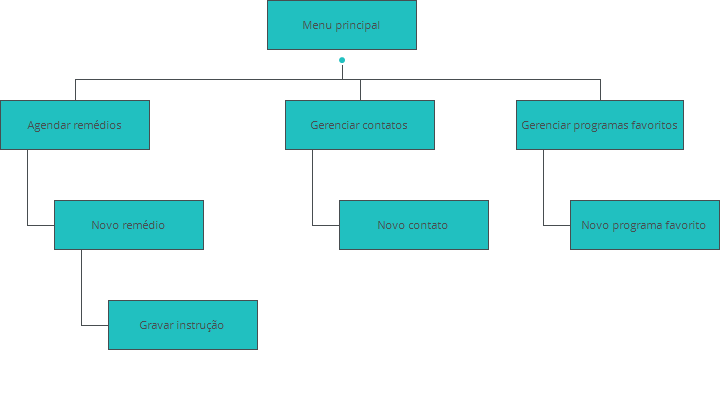
\includegraphics[width=1\textwidth]{prototipo.png}
\caption{Fluxo de telas do protótipo}
\end{figure}

\section{Projeto de software}

\subsection{Diagrama de classes}

\begin{figure}[h]
\centering
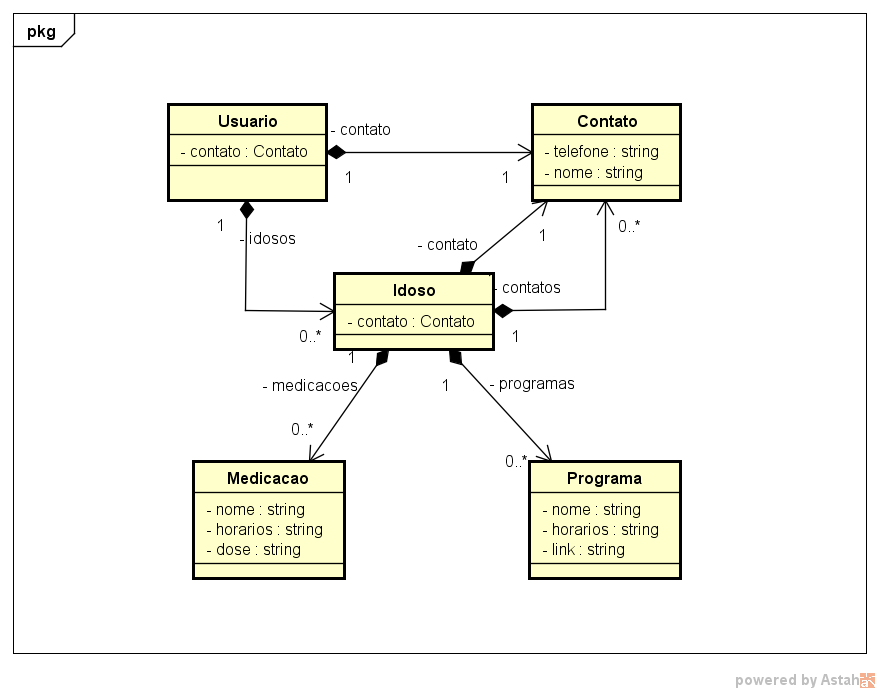
\includegraphics[width=1\textwidth]{classes.png}
\caption{Diagrama de classes}
\end{figure}

\subsection{Padrões de Projeto}

\subsection{Realm}


\section{Testes}